\chapter{Data-driven approach leveraging explicit feedback as target variable on Customer Satisfaction}
\label{ch:dataDriven}
Instead of using identified relevant features from the first approach to make predictions about a satisfaction level of customers, this approach should be fed with more features and find its way to the promising ones automatically. The goal was to work on a software framework which analyses data and selects the influential factors for Customer Satisfaction automatically while throwing away garbage data and redundant features. Furthermore, the lack of metrics in the data representing Customer Satisfaction identified as major issue during the first part of the thesis should be tackled by getting explicit feedback from customers on how satisfied they are. The expectation from this customer survey is that it provides a much more reliable quantitative measurement of the satisfaction level of a customer than any other kind of data Tractive collects in its database system. As described in more detail in the satisfaction theory part of chapter \ref{ch:backgroundResearch} understanding why a customer behaves in a certain way can be quite subjective, involve psychological factors and vary among different types of customers. Therefore it has to be admitted that this can hardly be extracted from some objectively collected data and the actual source of truth is to ask people themselves. With enough survey answers the framework should first analyse all observations retrieved by leveraging descriptive statistics and evaluate chances to predict satisfaction for arbitrary customers, who have not filled in the survey. With specific features selected machine learning algorithms can then be trained and evaluated on the data to find a model which is suited to do automated predictions. 

\section{Implementation of a survey to gather explicit feedback from customers}
Before any further data analysis task was started the initial task was to create a customer survey to collect usable information which gives a reliable insight into how a customer rates his experience with the product so far. A requirement was to keep the effort for the customer to fill in the survey low, which in first place means to require little time to fill in the duty part of the survey. Little time consumption correlates positively with response rate. According to \cite{reichheld2003one} customer surveys are often too complex and as a result overwhelming for the user even though the company cannot derive better decision from it. With regard to customer satisfaction and loyalty \cite{reichheld2003one} claim that the most essential number is the willingness of a customer to recommend the product to a friend or colleague. This metric should be on a scale of 0-10 to allow a computation of the NPS (Net-Promoter-Score), a widely used score to constitute growth of a company. In collaboration with responsible people at Tractive it was decided to limit the number of questions to the following two which were used later on to establish the target attribute in the prediction framework.

\begin{enumerate}
	\item How satisfied are you with Tractive GPS? (Scale 1-5)
	\item How likely are you to recommend Tractive to a friend or colleague? (Scale 0-10)
\end{enumerate}

Next to the specifications of questions, the survey should be appealing, personalized and easy to use. The final landing page of the customer survey is shown in figure \ref{fig:customerSurvey}. 

\begin{figure}
	\centering
	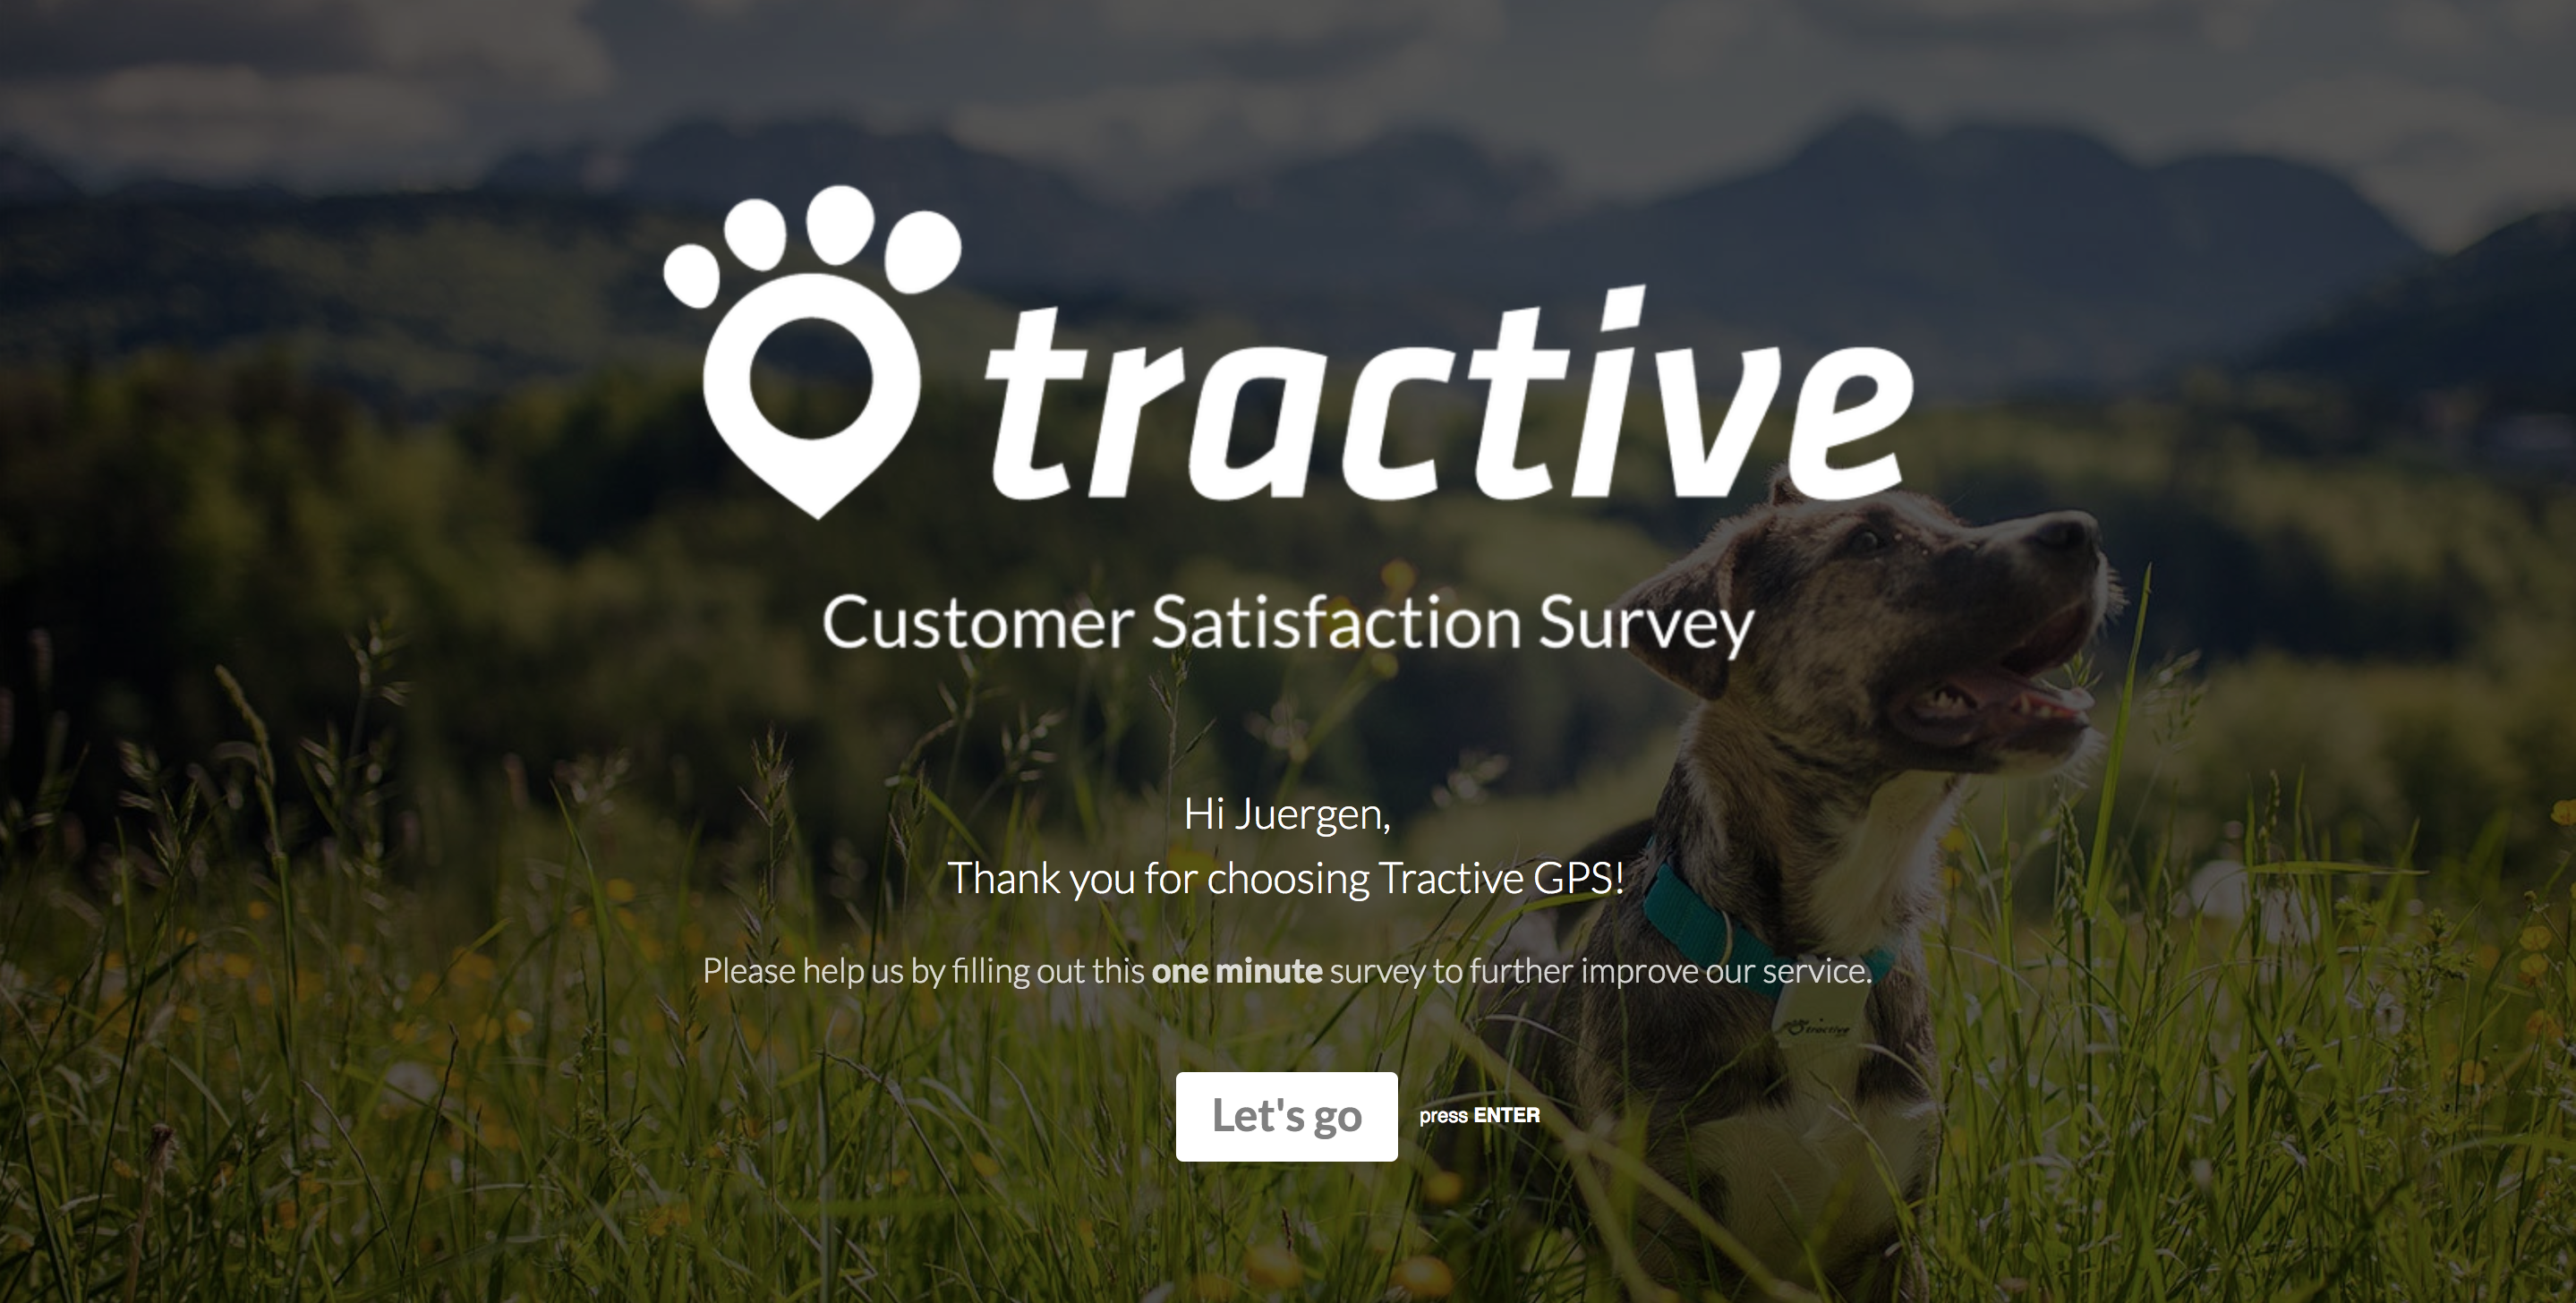
\includegraphics[width=0.8\textwidth]{img/customerSurvey.png}
	\caption{Customer Survey - Landing page}
	\label{fig:customerSurvey}
\end{figure} 

The goal of the company was to get customer feedback early on to be able to respond to unsatisfied customers quickly and in best case before they complain about a problem they have at customer support. As a result, the author of the thesis could arrange with the responsible people of Tractive to following procedure. When a new user converts successfully to a paying customer, he or she has to activate the GPS device before first usage. This enables the device to be actively used, sending positions and showing up on the map in the apps. Directly after activating the device, the backend service schedules an email in two weeks asking the customer to fill in the survey. To reach as many users as possible the survey was translated into the five major languages supported at Tractive, namely German, English, French, Italian and Spanish. Depending on the users stored demographical settings the correct language version is triggered. An example of how the email looks like is shown in figure \ref{fig:customerSurveyEmail}.

\begin{figure}
	\centering
	\includegraphics[width=0.8\textwidth]{img/customerSurveyEmail.png}
	\caption{Customer Survey - Email}
	\label{fig:customerSurveyEmail}
\end{figure} 

When the user clicks on the "Take Survey" button in the email, a browser window will open with the customer survey landing page. Behind the scenes In the URL (Uniform Resource Locator), the language version of the survey as well as the name of the customer is passed. For better personalization of the voluntary additional questions the name of the pet associated with the GPS device is sent as URL parameter. A necessary information is the unique id of the device since it allows to query all of the identified hardware- and position related data identified in section \ref{sec:dataSources}. For designing the customer survey the external tool Typeform was used. The following section describes briefly how the data gets extracted and integrated back into the internal database to be processable. Furthermore a few statistical details will be pointed out to get an impression with regard to the pending satisfaction analysis and prediction task.

\section{Results and interpretation of survey results}
\label{sec:surveyResults}
To fetch the survey results from Typeform, a nightly job was implemented which uses the provided API of Typeform and gets the results from the previous day. The essential metrics from the two duty questions are extracted and along with the user- , pet- and device data stored in a new collection in the main database of Tractive. A typical structure of a document in this collection is illustrated in table \ref{tab:surveyResponse}.

\begin{table}[]
	\centering
	\resizebox{\columnwidth}{!}{%
		\begin{tabular}{|l|l|l|}
			\hline
			\multicolumn{1}{|c|}{\textbf{Attribute}} & \multicolumn{1}{c|}{\textbf{Datatype}} & \multicolumn{1}{c|}{\textbf{Description}} \\ \hline
			\_id & ObjectId & Unique identifier of document \\ \hline
			survey\_id & String & Typeform identifier for the particular language version \\ \hline
			submit\_date & DateTime & Date and time when customer submitted survey \\ \hline
			user\_id & ObjectId & Reference to the user \\ \hline
			tracker\_id & ObjectId & Reference to the device \\ \hline
			rating & Integer & Overall satisfaction (scale: 1-5) \\ \hline
			recommendation\_score & Integer & Recommendation potential (scale: 0-10) \\ \hline
		\end{tabular}%
	}
	\caption{Structure of a survey response represented in the company database}
	\label{tab:surveyResponse}
\end{table}

The rating and recommendation score are the two interesting numbers when it comes to predicting satisfaction for an arbitrary user afterwards. The customer survey was deployed to the productive environment on 03.07.2017 which yielded the first survey result submitted on 17.07.2017. As of 28.10.2017 17:42 following statistics regarding the survey could be extracted.

\begin{itemize}
	\item Number of customer survey emails sent: 15695
	\item Number of customers who filled in the survey: 2182
	\item Percentage of users who filled in the survey: 13.9\%
\end{itemize}

As these numbers show, the response rate of the customer survey fortunately is quite good. The collected amount of customer survey data so far should be sufficient for finding potential patterns in the data. In order to get a better understanding some descriptive statistic values for the satisfaction rating and the value indicating willigness of a customer to recommend Tractive were calculated. The results are shown in table \ref{tab:statisticDescriptive}. 

\begin{table}[]
	\centering
	\resizebox{\columnwidth}{!}{%
		\begin{tabular}{|c|c|c|c|c|c|c|c|c|}
			\hline
			\textbf{Survey metric} & \textbf{Min.} & \textbf{1. Quartile} & \multicolumn{1}{l|}{\textbf{Median}} & \multicolumn{1}{l|}{\textbf{Mean}} & \multicolumn{1}{l|}{\textbf{3. Quartile}} & \multicolumn{1}{l|}{\textbf{Max.}} & \multicolumn{1}{l|}{\textbf{Variance}} & \multicolumn{1}{l|}{\textbf{Standard dev.}} \\ \hline
			Satisfaction & 1 & 3 & 4 & 3.688 & 5 & 5 & 1.327 & 1.152 \\ \hline
			Recommendation & 0 & 6 & 8 & 7.137 & 9 & 10 & 7.574 & 2.752 \\ \hline
		\end{tabular} %
	}
	\caption{Statistical summary - Overall satisfaction and recommendation score}
	\label{tab:statisticDescriptive}
\end{table}

Based on the results it can be followed that the average customer rates his or her satisfaction with the Tractive GPS product as mostly satisfied represented by a value close to 4. Similar is the recommendation likeliness value where the average lies between 7 and 8. Since the first quartile with a value of 6 is rather high, it can be followed that 75\% of the customers are more likely to recommend Tractive to a friend or colleague. To close this statistical analysis of survey responses it can be stated that the majority of customers tend to be satisfied which had to be considered accordingly in the prediction framework outlined in more detail in the following section \ref{sec:predictionFramework}.

\section{Software architecture and implementation of prediction framework}
\label{sec:predictionFramework}
This chapter provides detailed insights into the architecture and implementation of a Customer Satisfaction prediction framework leveraging introduced data mining techniques from section \ref{ssec:bottomUp}. Based on the data extracted by the implemented tool outlined in the previous chapter, it was the goal to train a suitable machine learning model on this data of users who answered the customer survey and increase the certainty of satisfaction outcome. As common in nearly any machine learning task, intensive experimenting in order to achieve good results is inevitable. Therefore the author tried to automate those experiments. Before elaborating on the individual components of the prediction framework, figure \ref{fig:frameworkOverview} provides a broad overview.

\begin{figure}
	\centering
	\includegraphics[width=0.8\textwidth]{img/frameworkOverview.png}
	\caption{Overview on the prediction framework}
	\label{fig:frameworkOverview}
\end{figure} 

\subsection{Preparing training data}
As the relevant data to analyze has already been queried with the implemented data extraction tool introduced in the last chapter, big parts of the implementation could be reused to prepare the training data for the prediction framework. However in contrast to the selection of random samples, it was necessary to limit the selection of the data to customers who had filled in the survey before. Therefore the first step was to query user and subscription data for those, including the user- and device ID in order to match the usage data queried later. In contrast to the hypotheses-driven approach where extracted data rows were confronted with each other to analyze them with statistical methods, the data was combined to large CSV file, which is the default input format for machine learning algorithms. Therefore, a data expansion function was implemented which passes gathered data to the next MongoDB aggregation task and combines queried data as new column in the CSV file. A short code extract of the combiner function is shown in listing \ref{lst:csvTrainingData}. 

\begin{lstlisting}[caption={Expanding CSV data with results from MongoDB aggregation queries}, label={lst:aggregationServerCommands}]
async.waterfall([
async.apply(user.insertUserData, customerSurveyData),
subscription.insertSubscriptionData,
customerSupport.insertCustomerSupportData,
device.insertDeviceData,
shareData.insertReceivedSharesForUsers,
shareData.insertSentSharesForTrackers,
resourceData.insertResourceData,
resourceSocialData.insertResourceCommentsData,
resourceSocialData.insertResourceLikesData,
notificationData.insertNotificationsData,
geofenceData.insertGeofenceData,
geofenceReportData.insertGeofenceReportData,
posReport.insertPosReportData,
idReport.insertNumberOfDaysInUse,
serverCmd.insertServerCmdMetricsData,
appUsageData.insertAppUsageData,
hwMetricsData.insertAverageBatteryLifeTime
], cb);
\end{lstlisting}

As introduced in the code listings from section \ref{sec:extractionTool}, the async library comes in handy here again to pass an array of JSON objects along each callback in a function. This way it can be used as "hidden" input parameter in each function. Finally, the expanded JSON array gets written to a CSV file. 

\subsection{Process training data and learn a classifier}
After having prepared the raw data, the empirical work continued with the implementation of the actual prediction framework. It was decided to develop a Java application and use the open source data mining software Weka implemented and maintained by the University of Waikato in New Zealand. Based on the theory of a comprehensive KDD process as outlined by \cite{fayyad1996data} and \cite{neckel2015}, the software architecture of the framework was designed similar to a pipeline where the data flows through and gets modified at each station. The final step in this pipeline was to learn a model based on different classifier algorithms and evaluate them. The fact that survey results were collected only two weeks after a customer had activated a device, some of the attributes have invalid values among several data observations. Moreover the ratio between satisfied and dissatisfied customers is about $1.875:1$. This led to a more difficult situation and required sophisticated methods in pre-processing. Figure \ref{fig:softwareArchitecture} illustrates a sketch of the software architecture. Afterwards the individual parts shown in the figure will be explained. The thesis then dives into the implementation details with Java and Weka.

\begin{figure}
	\centering
	\includegraphics[width=0.8\textwidth]{img/softwareArchitecture.png}
	\caption{Software architecture of the prediction framework}
	\label{fig:softwareArchitecture}
\end{figure} 

Before moving on, the essential Weka terminology should be briefly introduced to prevent any confusion afterwards. An in-memory data set in Weka is represented by the Instances object. A single data observation is called Instance and can be retrieved by calling dataSet.enumerateInstances(). Similarly, features can be accessed via dataSet.enumerateAttributes() whereby a feature in Weka terms is named Attribute. Next to a large set of different classification algorithms, Weka provides different useful filters for data pre-processing- and transformation as well as algorithms for feature selection. 

\subsubsection{FileProcessingEngine}
The task of this first component is to read the CSV outcome from the data extraction tool and convert it into the required format, namely ARFF (Attribute Relation File Format), which Weka is able to work with. The ARFF format is very similar to CSV except that it contains metadata describing the type and value range of each feature (called attribute in terms of Weka). To read in the CSV file and return so called Weka Instances, representing the data set in-memory, the ConverterUtils from Weka were used. The resulting raw data set is then passed on to the pre-processing station. Furthermore, the FileProcessingEngine implements a method to write a current data set to an ARFF file which is used to store intermediate results. Listing \ref{lst:fileProcessingEngine} shows the implementation of those methods. 

\begin{lstlisting}[caption={Implementation of FileProessingEngine}, label={lst:fileProcessingEngine}]
public static Instances readDataSetFromFile(String filename) {
	try {
		DataSource source = new DataSource(filename);
		return source.getDataSet();
	} catch (Exception e) {
		throw new RuntimeException("Data set could not be loaded from passed filename", e);
	}
}

public static void writeDataSetToFile(Instances dataSet, String filename) {
	try {
		ArffSaver arffSaver = new ArffSaver();
		arffSaver.setInstances(dataSet);
		arffSaver.setFile(new File(filename));
		arffSaver.writeBatch();
	} catch (Exception e) {
		throw new RuntimeException("Data set could not be written to file", e);
	}
}
\end{lstlisting}

\subsubsection{PreProcessingEngine}
The goal of this component is to prepare the data set in a way to build the best possible model when training a classifier at a later stage. Putting the raw data set from the FileProcessingEngine into a classification algorithm would lead to poor results as the quality of data for some features turned out to be bad. A view onto the statistics reveals that some attributes have a remarkable percentage of missing values. The features were grouped into smaller categories and are illustrated in table \ref{tab:preprocessingStatistics}.

\begin{table}[]
	\centering
	\begin{tabular}{|l|l|}
		\hline
		\textbf{Feature}         & \textbf{Missing values} \\ \hline
		Support ticket metrics   & 68\%                    \\ \hline
		Battery lifetime & 83\%                    \\ \hline
		Command duration         & 10\%                    \\ \hline
		Command delays           & 6\%                     \\ \hline
	\end{tabular}
	\caption{Missing values for some features}
	\label{tab:preprocessingStatistics}
\end{table}

The reason why there are missing values for these features can be explained as following. As expected upfront there are not that many customers, who have contact with the company support team. Thus, 68\% of customers have a ticket count of 0 and as a consequence missing support ticket metrics. Despite that, there is data available for about $1/3$ of customers who filled in the survey which allows some separate analysis later on. Since the calculation of hardware metrics started later, there is no battery lifetime data available for most of the devices from customers which gave satisfaction feedback. Although not that extreme, also the server command duration values are missing for some data observations most likely due to the short time span between activating the tracker and filling in the survey. This indicates that some users have not yet enabled live tracking at least once a time or did not have any successful live tracking so far. From these findings it can be concluded that missing data falls into the category of NMAR (Not-Missing-At-Random) as it was explained in the background research in section \ref{sssec:explorationData}. Techniques proposed in the theory were implemented to handle those missing values. Following paragraphs take a look on the implementation details. 

\paragraph{Filter unneeded features manually}
Although the author could not exclude any particular features based on the statistical analysis from the previous chapter, the ticket metrics and the battery lifetime cannot contribute anything positive to learn a reliable model due to the large amount of missing values. They rather distort the learned model and thus have negative impact. Therefore it was decided to remove all features which exceed a defined threshold of missing values completely from the data set. With the RemoveFilter from Weka the features can be removed from the data set contained in the passed Instances object. As applying a Weka filter is a repetitive action, it was implemented as utility method in the Utils class. Code listing \ref{lst:removeUnneededFeatures} shows an example of how to remove unneeded features which have more than 25\% missing values.

\begin{lstlisting}[caption={Remove unneeded features}, label={lst:removeUnneededFeatures}]
public static Instances filterAttributesWithTooManyMissingValues(Instances dataSet) {
	return filterAttributesNotFulfillingCriteria(dataSet, attribute -> {
		int numberOfMissingValues = (int) Collections.list(dataSet.enumerateInstances())
			.stream()
			.filter(instance -> instance.isMissing(attribute))
			.count();
		float missingValuesPctg = ((float) numberOfMissingValues / dataSet.numInstances());
		return missingValuesPctg > 0.25;
	});
}
private static Instances filterAttributesNotFulfillingCriteria
(Instances dataSet, Predicate<Attribute> criteria) {
	String[] attributeNamesToRemove = Collections.list(dataSet.enumerateAttributes())
		.stream()
		.filter(criteria)
		.map(Attribute::name).toArray(String[]::new);
		
	return filterUnneededAttributes(dataSet, attributeNamesToRemove);
}
private satic Instances filterUnneededAttributes(Instances dataSet, String[] attributeNames) {
	Remove removeFilter = new Remove();
	removeFilter.setAttributeIndicesArray(getAttributeIndices(dataSet, attributeNames));
	return Utils.applyFilter(dataSet, removeFilter);
}
\end{lstlisting}

\paragraph{Filter features with no variance}
The variance of numeric features was investigated to filter extreme cases which show no variance at all. To overcome this problem those features were removed as well from the data set. The filterAttributesNotFulfillingCriteria method shown in the previous code listing was reused here with a different predicate function passed. Algorithm \ref{lst:removeAttributesNoVariance} shows how this was implemented.

\begin{lstlisting}[caption={Remove features}, label={lst:removeUnneededFeatures}]
public static Instances filterAttributesWithNoVariance(Instances dataSet) {
	return filterAttributesNotFulfillingCriteria(dataSet, attribute ->
		attribute.isNumeric() && dataSet.variance(attribute) == 0.0);
}
\end{lstlisting}

\paragraph{Imputation of missing values}
As indicated earlier in this section, 5-10 \% of the server command data collected showed missing feature values. In contrast to the cases considered before, these features could not be simply removed from the dataset as they too much important information regarding Customer Satisfaction. The categorical analysis in section \ref{sec:hypothesesDriven} showed for a small random sample a statistical significant evidence that the live tracking success rate influences customer churn. It was decided that this feature has to be kept for the data mining stage. As a result, the best possible technique was imputing the missing values accordingly. First of all, the imputation was done with the mean value of the feature under consideration. This method is available only for numeric attributes which was fine in this situation as the server command related data only consists of numeric features. Extracts of the implementation are shown in listing \ref{lst:meanImputation}.

\begin{lstlisting}[caption={Mean and mode imputation of missing values}, lable={lst:meanImputation}]
private static Instances replaceMissingAttributeValues(Instances dataSet, Set<Attribute> replaceableAttributes) {
	if (!replaceableAttributes.stream().allMatch(Attribute::isNumeric)) {
		throw new RuntimeException("Not all attributes to replace with the replacement value are numeric");
	}
	Enumeration<Instance> instanceEnumeration = dataSet.enumerateInstances();
	
	while (instanceEnumeration.hasMoreElements()) {
		Instance instance = instanceEnumeration.nextElement();
		
		for (int i = 0; i < instance.numAttributes(); i++) {
			Attribute currentAttribute = instance.attribute(i);
			if (instance.isMissing(i) && replaceableAttributes.contains(currentAttribute)) {
				instance.setValue(currentAttribute, getReplacementValue(dataSet, currentAttribute));
			}
		}
	}
	return dataSet;
}

private static double getReplacementValue(Instances dataSet, Attribute attribute) {
	return Collections.list(dataSet.enumerateInstances())
		.stream()
		.filter(instance -> !instance.isMissing(attribute))
		.collect(Collectors.averagingDouble(x -> x.value(attribute)));
}
\end{lstlisting}

Next to the input data set the method takes as second parameter a set of features to replace with the mean value. First of all the method asserts whether all features to replace are numeric, otherwise an exception will be thrown. Within the subsequent while loop the features to replace are searched and the value gets substituted by a replacement value, calculated in getReplacementValue(dataSet, currentAttribute). This method iterates over all instances and calculates the arithmetic mean among the present values for the current feature.

% TODO: If I have implemented a different imputation method, add the documentation here

\paragraph{Defining the Weka class attribute}
After reading in the raw data from the CSV file, Weka does not know which of the features is used as class attribute needed to perform a classification task. The class attribute is the ground truth value for each data observation in the training set a classification algorithm uses for learning and evaluating a model. The important metrics provided by the survey results are the overall satisfaction level on a scale from 1-5 and the recommendation potential on a scale from 0-10. As the gathered experience from theory and hypotheses-driven testing at this point in time showed the difficulty of deriving relationships between certain features and Customer Satisfaction, it was decided to make the class value binary, namely satisfied or dissatisfied. With regard to business requirements it made sense to claim that below a rating of 4 customers tend to be dissatisfied while a value of 4 and 5 means that the customer tends to be satisfied. A similar machine learning approach for Customer Satisfaction, documented by \cite{meinzer2016can}, which was mentioned in the related work section did the same satisfaction level classification and thus confirms the thoughts. Therefore, in advance of marking the feature as class attribute it had to be normalized accordingly. 




 



